\documentclass{article}
\usepackage[english]{babel}
\usepackage[utf8]{inputenc}
\usepackage[T1]{fontenc}
\usepackage{hyperref}
\usepackage[margin=0.5in]{geometry}
\usepackage{xspace}
\usepackage{xcolor}
\usepackage{amsmath}
\usepackage{graphicx}
\usepackage{palatino}
\usepackage{microtype}

\title{Susceptible-Infected Models for Spatial Vector-Borne Disease}
\author{Drew Dolgert}
\date{\today}


\begin{document}
\maketitle

\section{Introduction}
Approximately seven million people have Chagas disease. It's important.

The causative agent for Chagas disease, T.\ cruzi, is spread by
an insect called Triatoma infestans. The basic model is that 
T.\ infestans spreads Chagas among people and animals in a house.
In order for another household to catch the disease, either people
or the T.\ infestans travel to neighboring houses.
There are three levels, behavior of people, infestation by
T.\ infestans, and spread of T.\ cruzi by T.\ infestans and people.

Mike Levy's group has collected excellent data on the spread of
T.\ infestans in a city. The data are observations of the observed
abundance of insects in households, taken during different sweeps.
All of the work to record abundance amounts to a partially-observed
single trajectory of the system, taken as a whole.

Given that single trajectory of the T.\ infestans through a city,
we would like to ask how behaviors of the insects affect spread
of infestation because this could help intervention against
T.\ infestans. Mike Levy's group previously published a paper
which observed clustering of observations within city blocks,
indicating the insects are less likely to cross roads when
they emigrate a house.

Now we would like to infer from the observed trajectory
to what extent roads affect bug movement. That is a spatial
trajectory defined by bug movement. It is one trajectory
among a combinatorial number of ways T.\ infestans could spread
through the city. We don't have a likelihood for that trajectory,
but we could write a likelihood for an equivalent simplified model.

The simplified model assigns to each house either the state
susceptible or the state infested. Spread from house to house
is assumed to have a uniform hazard within a cutoff distance
and a much smaller hazard at distances greater than the cutoff.
This simplified model, dubbed hop-skip-jump, is a maximum
entropy assumption.

Our concern is that a model which labels the state of the
house will combine several insect behaviors into more
coarse-grained house-infestation behaviors, smearing out
how insect vector movement affects where infestation spreads.
We want to distinguish movement of bugs from stochastic
die-off of populations of T.\ infestans in a house.

This article constructs the simplified \textsc{si} model
rationally from a model of individual T.\ infestans. It uses
a Verhulst model for the insects and establishes a projection
to the more coarse-grained \textsc{si} description.


%%%%%%%%%%%%%%%%%%%%%%%%%%%%%%%%%%%%%%%%%%%%%%%%%%%%%%
\section{Models}
\subsection{Hop-skip-jump Movement Model}
MaxEnt in space, with a choice for normalization.

How to add streets.

\begin{figure}
\centerline{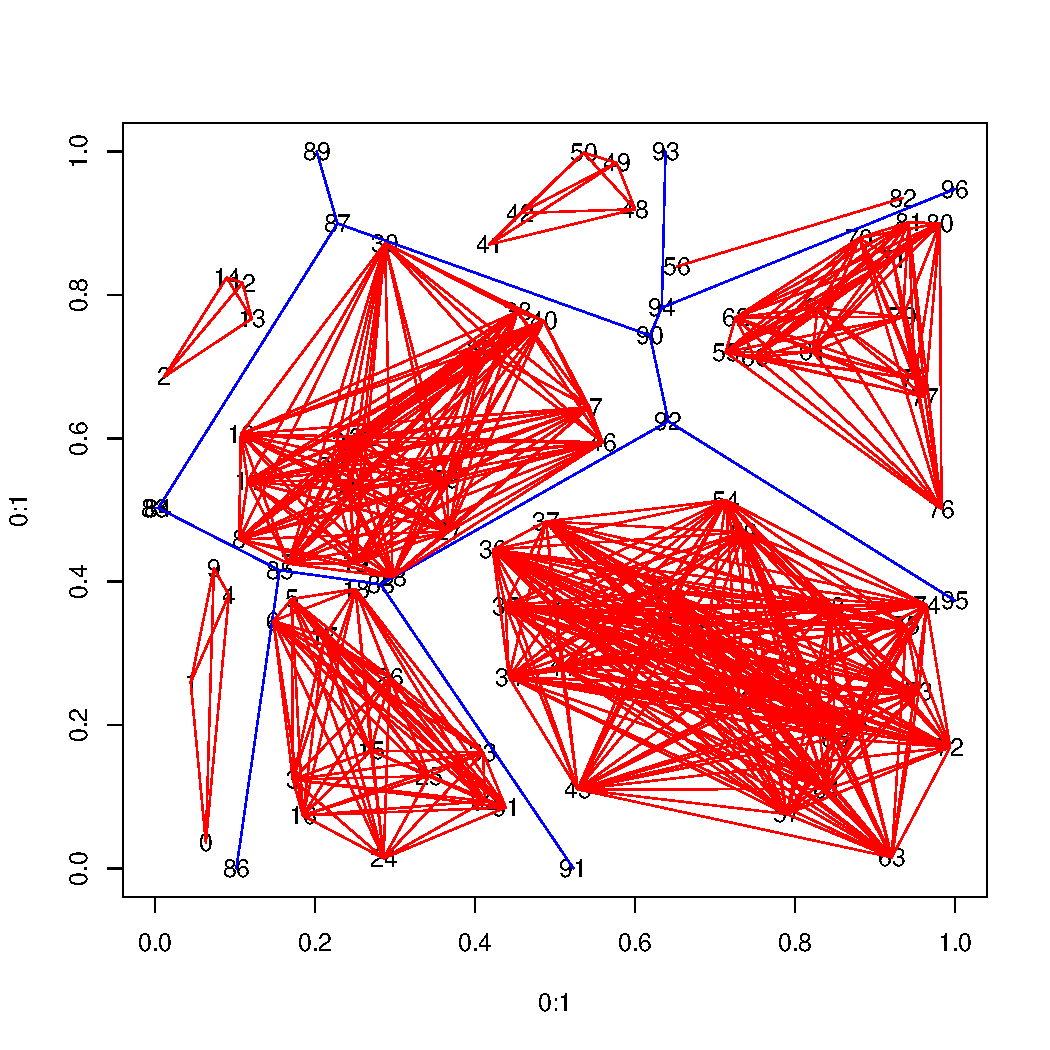
\includegraphics[width=10cm]{blocks.pdf}}
\caption{Houses on different blocks are separated by streets.
Calculate the number of streets crossed by walking house-to-house.\label{fig:blocks}}
\end{figure}

%%%%%%%%%%%%%%%%%%%%%%%%%%%%%%%%%%%%%%%%%%%%%%%%%%%%%%
\subsection{Explicit Spatial Vector Movement Model}
It would be possible to construct a colony growth and
vector movement model for T.\ infestans from expert opinion.
The goal of this article is to ask how to rationally project
any model of individual vectors onto a coarser model.
We choose an underlying vector model which preserves
our preference not to assume what we don't know.
The underlying model for bug birth and death will be
a Verhulst model. As described in N{\aa}sell\cite{Nasell2001},
the Verhulst model predicts logistic growth of bugs within
a house. This model has one more parameter than the
basic \textsc{si} model, effectively controlling variance in
bug growth.

What we gain by introducing a vector-based model with
almost as few parameters as the coarse-grained model is
that the behaviors of the vector provide inherent structure
to the coarse-grained model. Two specific examples
are the time-dependence of emigration and tendency for
stochastic die-off. Modeling birth
and death of insects will generate not only logistic
growth of a population infesting a house, but nearly-logistic
growth of individuals emigrating that house to form new
colonies. This time-dependence is inherent in the insect-based
model and important for early spread of infestation.
Stochastic die-off will decrease the rate of spread
to neighboring houses and may conflate with inference
about mobility of bugs.


\begin{figure}
\centerline{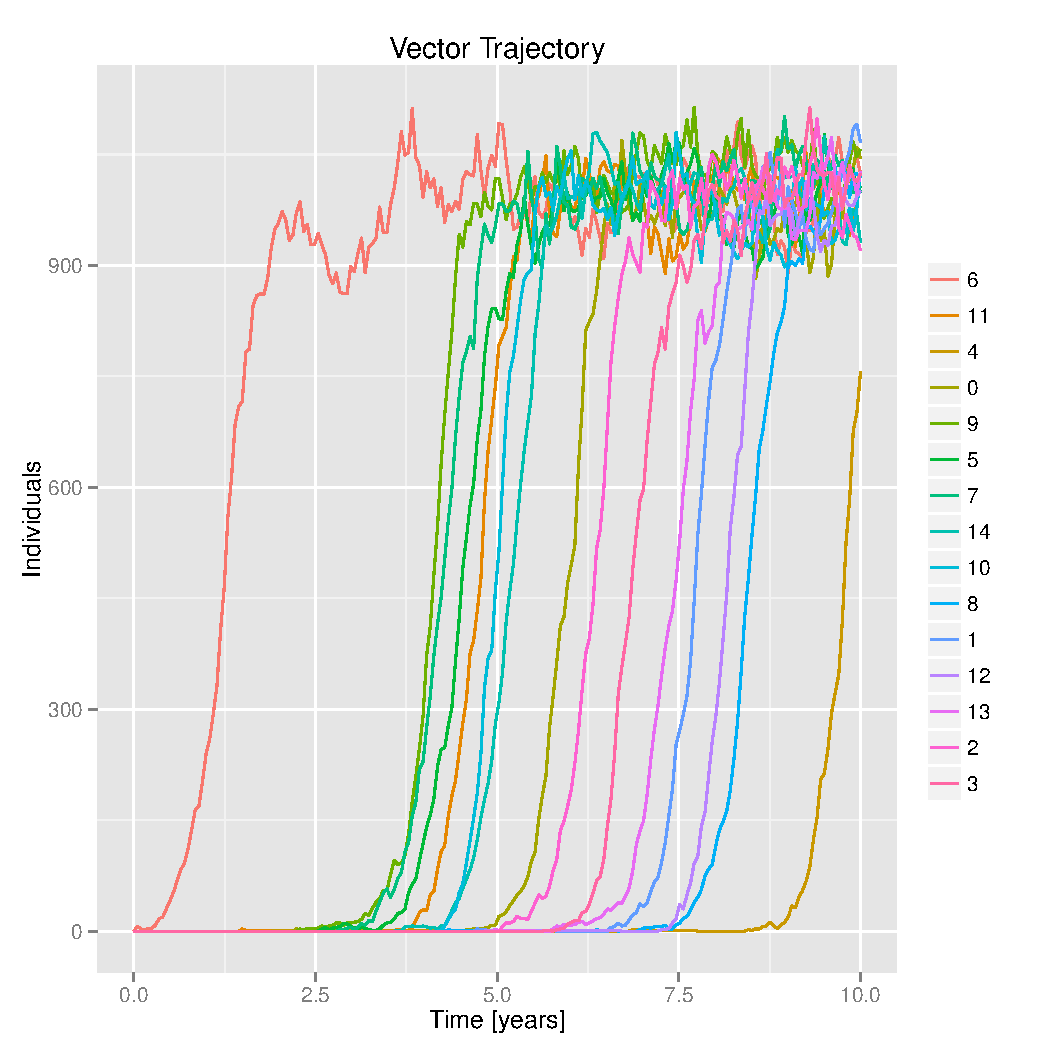
\includegraphics[width=10cm]{housecounts.pdf}}
\caption{For a small simulation of ten houses, the vectors increase in number one
individual at a time.\label{fig:housecounts}}
\end{figure}


\begin{figure}
\centerline{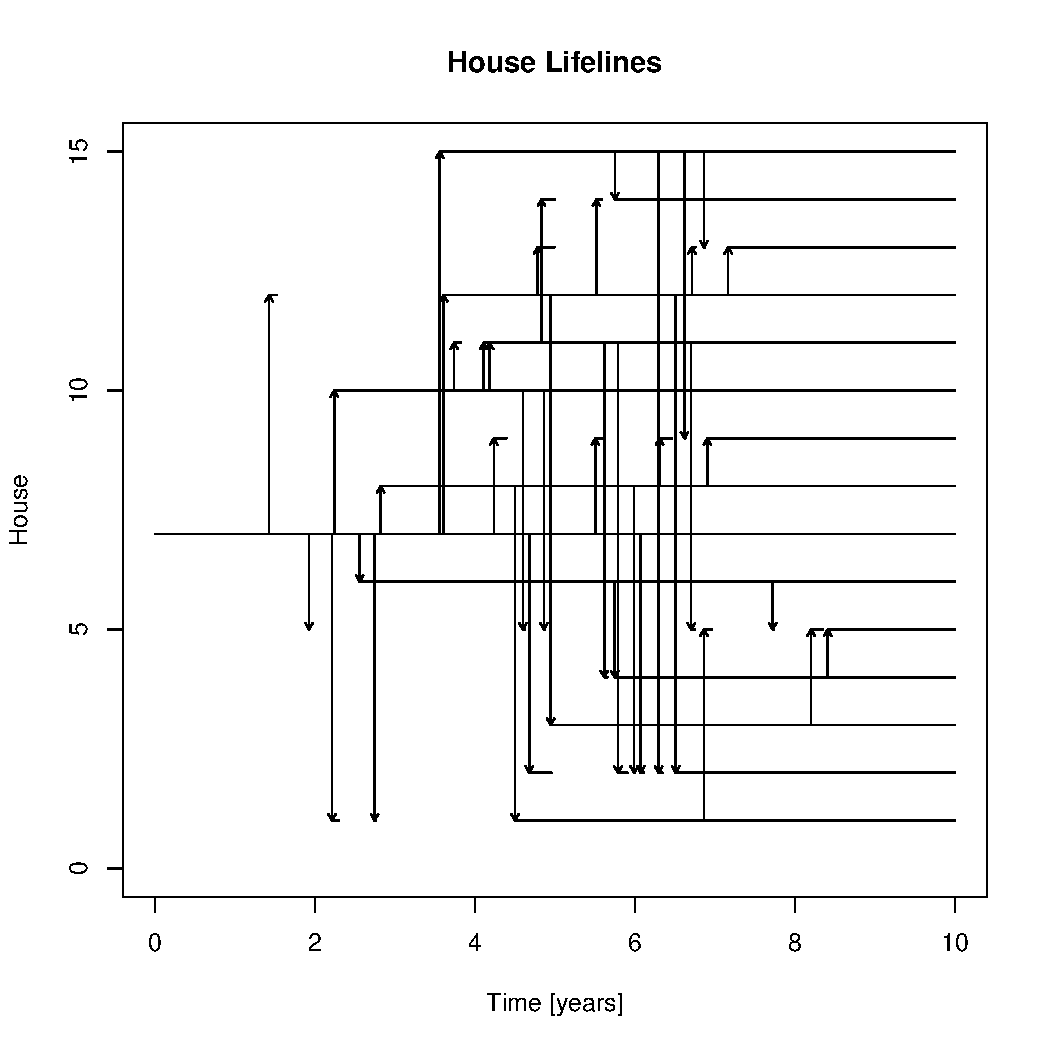
\includegraphics[width=10cm]{houselive.pdf}}
\caption{This shows when each house has any bugs in it.
The arrows indicate movement of a bug from one house to another.
Stochastic die-off is shown by lines ending.\label{fig:houselive}}
\end{figure}

%%%%%%%%%%%%%%%%%%%%%%%%%%%%%%%%%%%%%%%%%%%%%%%%%%%%%%
\subsection{Susceptible-infested House Model}



%%%%%%%%%%%%%%%%%%%%%%%%%%%%%%%%%%%%%%%%%%%%%%%%%%%%%%
\section{Coarse-Graining by Projection}
Given the model for behavior of individual vectors, construct a 
model for behavior of house infestations.

\begin{tabular}{ll}
Model & Projection \\
SI & A house is infested if vectors would last past stochastic die-off. \\
SIS & A house is infested if there is one bug. \\
SI & Constant hazard rate for infectiousness.
\end{tabular}

Fidelity of coarse-grained model over long times.
Fidelity of coarse-grained model for early outbreaks.



\section{Likelihood of Trajectory}
Given a measured trajectory, what is the likelihood using
a coarse-grained model, derived from the vector model?

\begin{itemize}
\item Using MLE on log-likelihood trajectories.
\item Using synthetic likelihood and MCMC.
\item Using ABC?
\end{itemize}


\bibliographystyle{plain}
\bibliography{vectored}
\end{document}
